% TeXiFy 似乎无法正确解析 main.tex 和 thesis-ref.bib 的关联,导致误报 UnresolvedReference
%! suppress = UnresolvedReference
\documentclass{ecnuthesis}
% 模版选项:
% printMode     是否开启打印模式, 若缺省则为关闭, 反之则为开启
% 用法示例
% \documentclass[printMode]{ecnuthesis}   (开启打印模式, 适合双面打印)
% \documentclass{ecnuthesis}              (关闭打印模式, 适合提交电子版)

\ecnuSetup {
% 参数设置
% 允许采用两种方式设置选项:
%   1. style/... = ...
%   2. style = { ... = ... }
% 注意事项:
%   1. 请勿在参数设置中出现空行
%   2. "=" 两侧的空格将被忽略
%   3. "/" 两侧的空格不会被忽略
%   4. 请使用英文逗号 "," 分隔选项
%
% info 类用于输入论文信息
    info = {
        title = {面向移动终端的可穿戴动态心电图的智能监测应用},
        % 中文标题
        %
        titleEN = {Intelligent Monitoring Application of Wearable Dynamic Electrocardiogram for Mobile Terminals},
        % 英文标题
        %
        author = {刘议临},
        % 作者姓名
        %
        studentID = {10195101428},
        % 作者学号
        %
        department = {软件工程学院},
        % 学院名称
        %
        major = {软件工程},
        % 专业名称
        %
        supervisor = {王丽苹},
        % 指导教师姓名
        %
        academicTitle = {副教授},
        % 指导教师职称
        %
        year  = 2023,
        % 论文完成年份
        %
        month = 4,
        % 论文完成月份
        %
        keywords = {\todo{todo}},
        % 中文关键词
        % 请使用英文逗号 "," 以分隔
        %
        keywordsEN = {\todo{todo}},
        % 英文关键词
        % 请使用英文逗号 "," 以分隔
        %
    },
% style 类用于简单设置论文格式
    style = {
        footnote  = plain,
        % 脚注编号样式
        % 可用选项:
        %   footnote = plain|circled
        % 说明:
        %   plain     脚注的编号仅为数字
        %   circled   脚注的编号为带圆圈数字 (仅限1-10)
        %   (默认选项为 plain )
        %
        numbering = arabic,
        % 章节编号样式
        % 可用选项:
        %   numbering = arabic|alpha|chinese
        % 说明:
        %   arabic    使用数字进行编号 (即理科要求)
        %   alpha     使用字母进行编号 (即外文要求)
        %   chinese   使用汉字进行编号 (即文科要求)
        %   (默认选项为 arabic )
        %
        fontCJK = fandol,
        % 中文字体选择
        % 可用选项:
        %   fontCJK = fandol|windows|mac
        % 说明:
        %   fandol    使用 TeX 自带的 fandol 字体
        %   windows   使用 Windows 系统内的字体 (中易)
        %   mac       使用 MacOS 系统内的字体
        %   (默认选项为 fandol )
        %
        fontMath = lm,
        % 数学字体选择
        % 可用选项:
        %   fontMath = lm|times
        % 说明:
        %   lm        使用 TeX 自带的 Latin Modern 数学字体
        %   times     使用 Times 风格的数学字体
        %   (默认选项为 lm )
        %
        bibResource = {./thesis-ref.bib},
        % 参考文献数据源
        % 由于使用的是 biber + biblatex , 所以必须明确给出 .bib 后缀名
        %
        logoResource = {./inner-cover(contains-font).eps},
        % 封面插图数据源
        % 模版已自带, 位于 ./inner-cover(contains-font).eps
        % 默认值为空
    }
}

% 需要的宏包可以自行调用
\usepackage[chapter]{easy-todo}
\usepackage{graphicx}
\usepackage{newfloat}
\usepackage{hyperref}

% https://tex.stackexchange.com/a/584994/254533
\captionsetup[figure][bi-second]{name=Figure}
\captionsetup[bi-second]{listtype+=Eng}
\DeclareFloatingEnvironment[fileext=lof2]{figureEng}[Figure][List of Figures]

\begin{document}

    \newcommand*{\app}{移动心电监测应用}


% 设置前置部分编号
    \frontmatter

% 中文摘要环境
    \begin{abstract}
        \todo{300到500字,要求概括地表述论文(设计)的研究背景、目的、研究方法、研究重点、结果和主要结论。}
    \end{abstract}

% 英文摘要环境
    \begin{abstractEN}
        \todo{中文摘要写完之后翻译一下}
    \end{abstractEN}

% 设置正文编号
    \mainmatter


    \chapter{绪论}\label{ch:intro}


    \section{\app 的背景与意义}\label{sec:background}

    \subsection{国内外心血管疾病现状}\label{subsec:disease}

    根据中国国家心血管病中心出版的《中国心血管健康与疾病报告2021》,目前中国人口心血管疾病的发病率和患病率均处于持续上升阶段,心血管疾病已成为居民死亡的首位原因;2019年,中国农村、城市心血管疾病分别占死因的46.74\%和44.26\%;心血管疾病给社会和居民带来的经济负担日益加重,且杀伤力越来越强\cite{Zhongguoxinxieguanjiankangyujibingbaogao20212022}。

    不仅如此,根据世界卫生组织的统计,心血管疾病也是全球的头号死因,每年死于心血管疾病的人数多于任何其它死因;2019年,估计有1790万人死于心血管疾病,占全球死亡总数的32\%\cite{CardiovascularDiseasesCVDs}。

    同时,近年来新型冠状病毒(COVID-19)的爆发也加剧了心血管疾病的危害。证据显示,既往合并心血管疾病的患者更容易在新型冠状病毒感染后发展为重症患者,死亡风险更高,预后更差\cite{zhangXinxingguanzhuangbingdufeiyanyuxinxieguanjibing2020}。

    \subsection{心电监测的用途与原理}\label{subsec:monitoring}

    尽早发现心血管疾病非常重要,这样就可以及时采取措施,减少疾病对患者健康的威胁\cite{CardiovascularDiseasesCVDs}。在各种心血管疾病的诊断方法中,心电图是最常用、最基本、最重要的一种,具有非侵入性、诊断快速、成本低廉、广泛可用等诸多优点\cite{Xinxieguanjibingzhenduanliuchengyuzhiliaocelue2007}。

    心电图(Electrocardiogram,缩写为ECG)是对心电信号的记录。通过放置在皮肤上的电极可以检测到心脏的电活动,将电压与时间的关系绘制为二维图像就得到了心电图,如图\ref{fig:10sec-ekg-lead}所示。

    \begin{figure}
        \centering
        % 这个大小刚好可以把 \subsection{静态与动态心电图} 挤到下一页,但不会把自己挤下去
        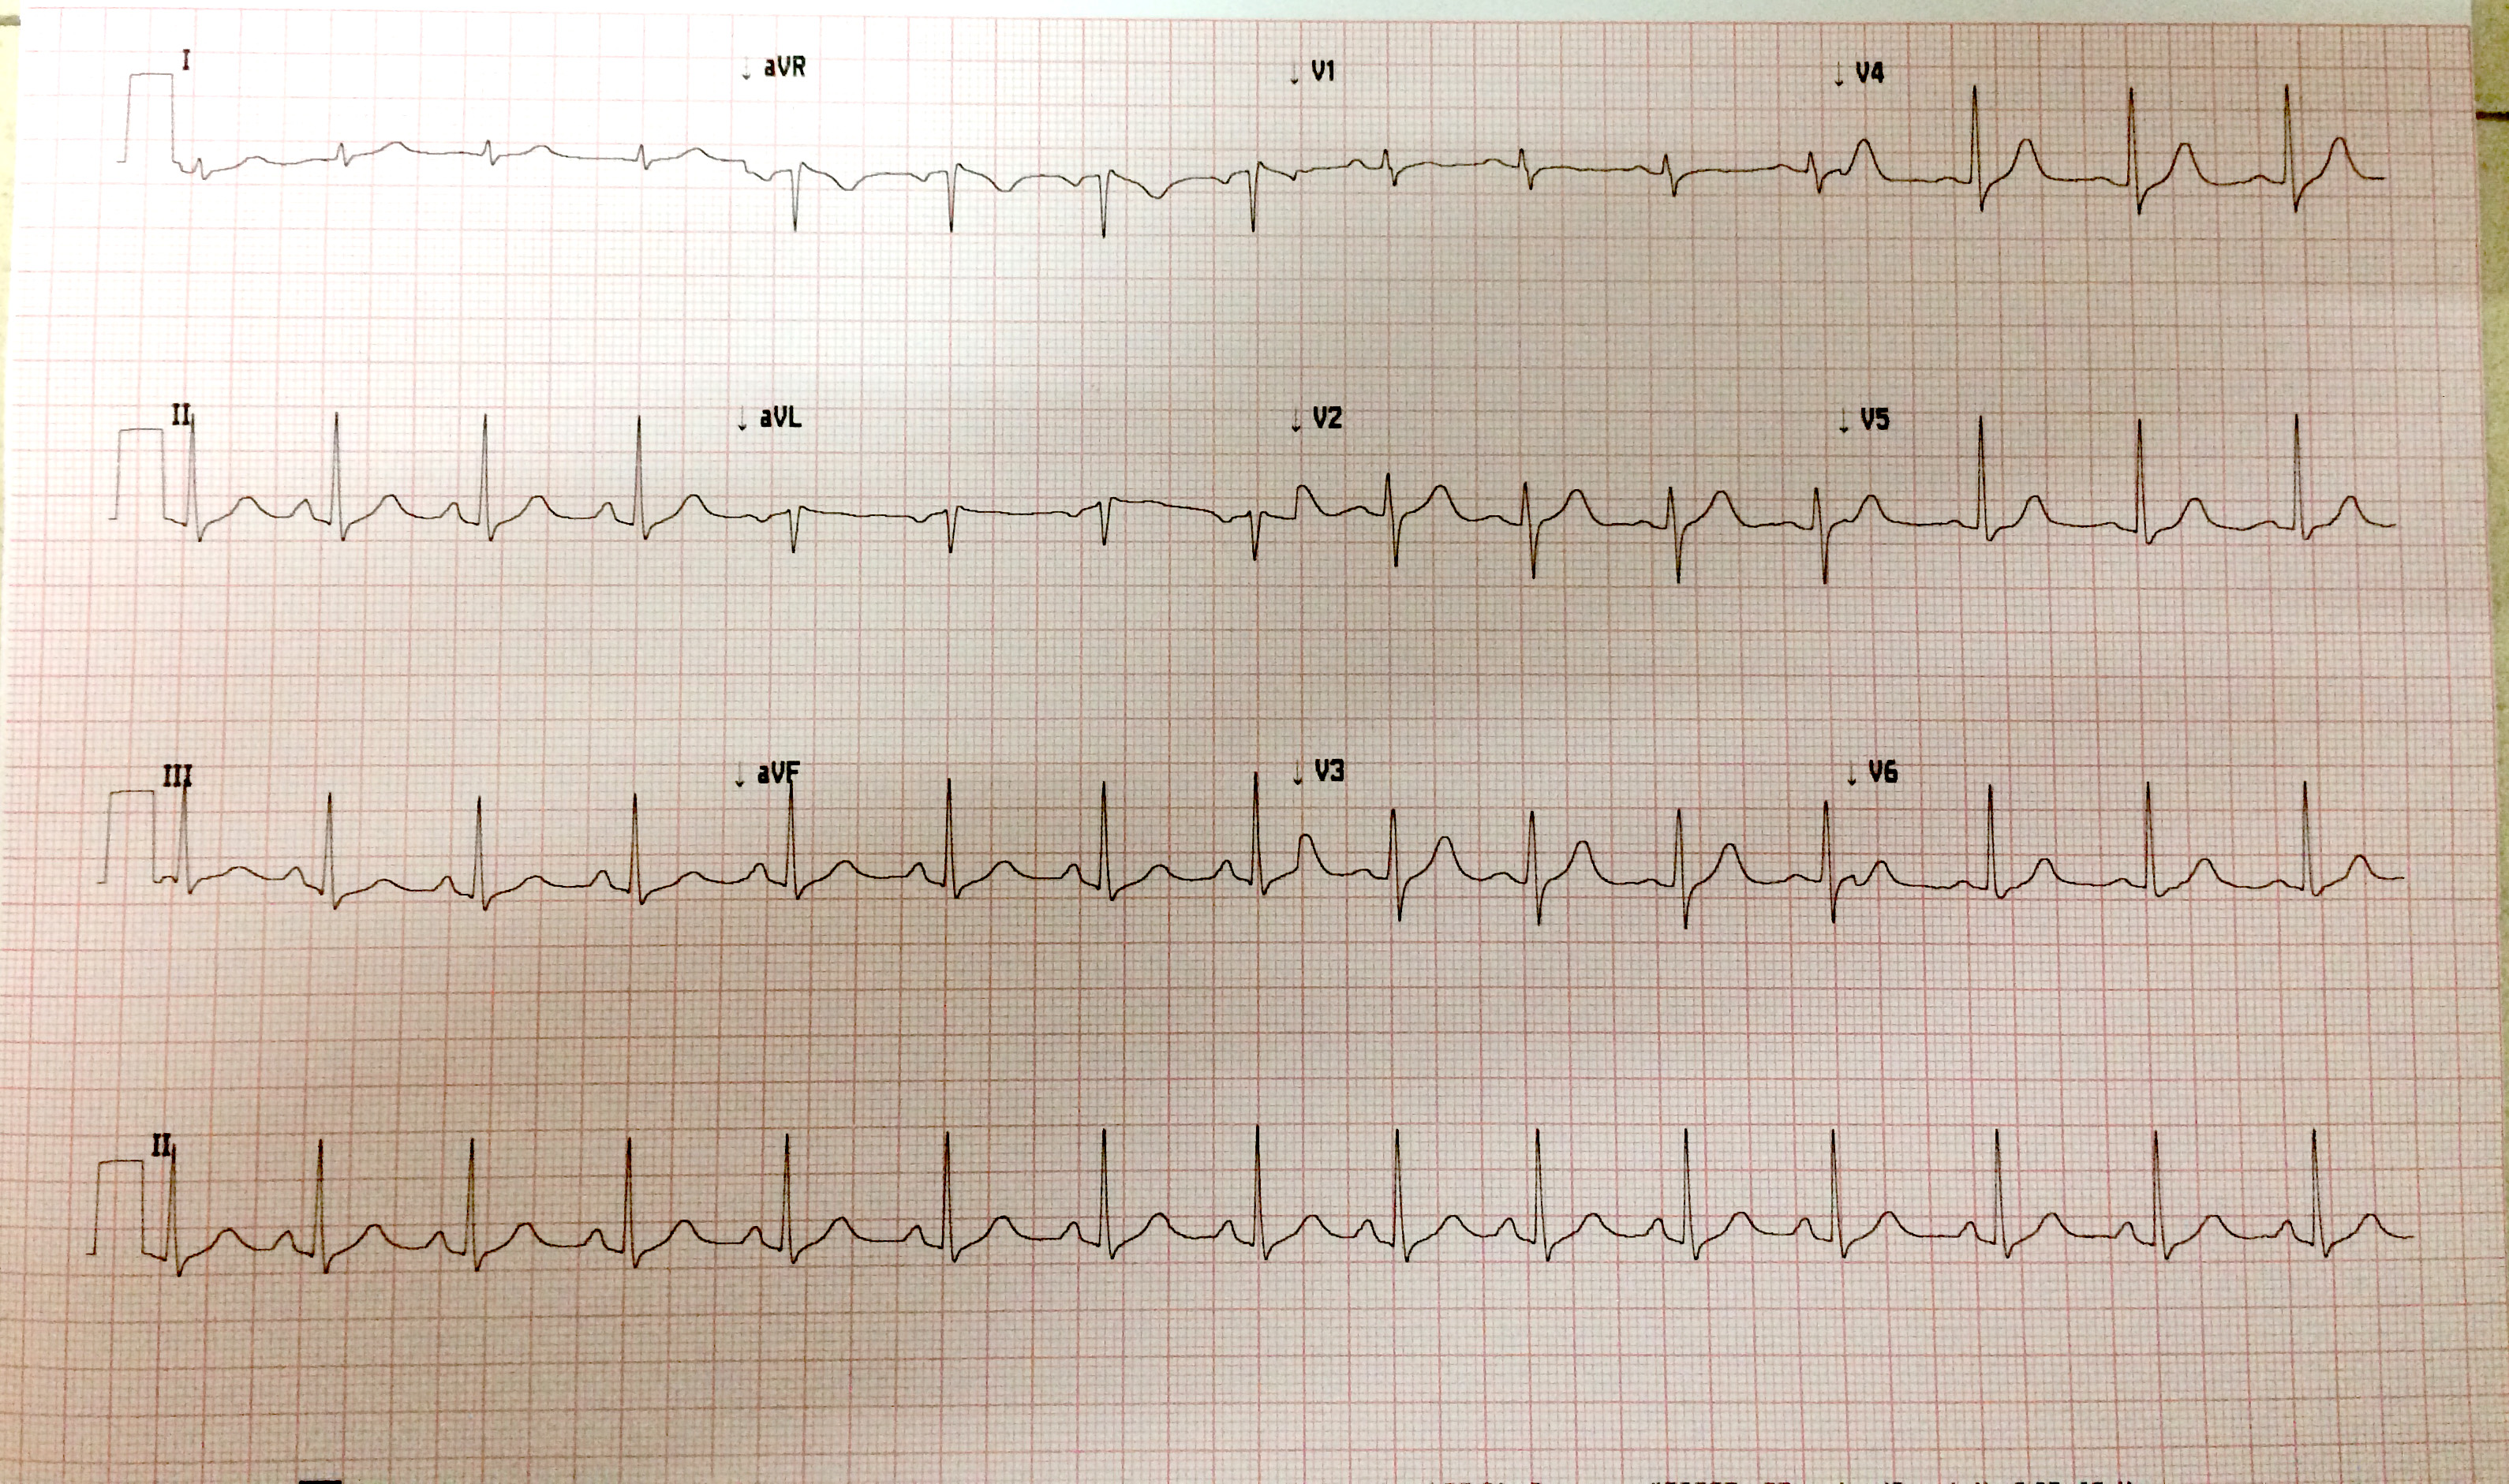
\includegraphics[width=.63\textwidth]{../assets/10sec-ekg-lead}
        \bicaption{一张10秒12导联心电图}{A 10-second 12-lead ECG}\label{fig:10sec-ekg-lead}
    \end{figure}

    \subsection{常规心电图与动态心电图}\label{subsec:standard-holter}

    \todo{什么是静态与动态心电图?}

    \todo{为什么需要日常的动态心电监测?}

    \subsection{心电自动诊断技术}\label{subsec:diagnosis}

    \todo{心电自动诊断技术的必要性,动态心电图数据量太大}

    基于可穿戴设备对心电数据进行实时分析可以及时发现患者的异常状况,为患者提供随时随地的医疗监护,降低心血管疾病对患者健康的威胁。

    \subsubsection{心电分割算法}\label{subsubsec:segmentation}

    \todo{todo}

    \subsubsection{心电分类算法}\label{subsubsec:classification}

    \todo{todo}

    \subsubsection{移动端心电自动诊断}\label{subsubsec:mobile}

    \todo{todo}


    \section{国内外\app 现状}\label{sec:status}

    \todo{相关研究领域的现状和研究进展分析,或与应用系统研发相关的技术发展现状}

    当前国内外已有不少基于可穿戴设备的远程心电监测系统,其中一些使用了手动编写的算法\cite{zhengJiyukechuandaishebeideyidongjianhuAPP2019,wuYidongxindianjiancexitongdeyanjiuyushixian2018,chenYidongxindianxinxijianhuxitongjixindianjiancesuanfadeyanjiu2018,heJiyuyidongpingtaidexindianjianceyiliaoxitongdeshixian2017,gradlRealtimeECGMonitoring2012,wenRealtimeECGTelemonitoring2008},另一些则使用了机器学习技术。使用机器学习技术的系统大致可以分为两类:一类是在移动端只对数据进行简单统计,完整的算法模型则部署于服务端\cite{wangJiyushenduxuexideyidongyuanchengxindianjiancexitongshejiyushixian2020,singhSmartECGMonitoring2022}。患者如果想获取完整的分析报告,则需要将数据上传至服务端后,等待服务端分析完成。在这类系统中,患者能在移动端立即获取的结果较少,而完整分析结果可能因为网络质量差、服务端算力不足等原因而有较大延迟。另一类则是边缘计算架构,将模型部署在移动端,数据分析直接在移动端进行\cite{chenJiyushenduxuexidexindianfenximoxingdeshejiyuyouhua2021,liuJiyuyidongzhongduanfenxidekechuandairouxingxindianjiancexitong2021,wangEnablingSmartPersonalized2014,jinPredictingCardiovascularDisease2009}。这样可以缩短延迟,节省带宽,并节省了高算力服务器的成本。但已有的少数此类应用都只实现了极简单的功能,旨在以演示程序验证模型正确性,并没有进行完整的应用开发。此外,此类演示程序均只进行了Android平台的开发。


    \section{本项目的主要工作}\label{sec:work}

    \todo{
        本选题与现有研究工作或应用系统之间的区别。
        本选题的主要研究内容、重点和特点,着重论述学生本人将完成的工作。
        论文预期达到的目标,包括提出的新方法或新技术、对现有技术的改进、或所研发系统的功能等内容。
    }

    本选题与上述最后一类系统相似,与已有应用系统的主要区别在于两点:其一是包含较完整的产品功能,可以投入到实际使用中;其二是基于跨平台开发框架,同时支持Android平台和iOS平台的移动设备。课题的选题来源于导师心电图课题的子项目,该课题目前已基于PyTorch训练了心电数据分类模型,并使用Python编写了相关算法,下一阶段的目标是将模型部署至移动端,课题目标明确,并已经具备较好的人工智能算法模型的技术支撑。


    \section{论文组织结构}\label{sec:structure}

    \todo{todo}


    \chapter{相关技术分析与介绍}\label{ch:tech}

    \todo{技术方案(技术路线、技术措施),包括应用系统的架构和开发环境}


    \chapter{\app 的需求分析}\label{ch:requirement}

    \todo{todo}

    本应用的目标用户是佩戴可穿戴心电信号监测设备的院外患者,以中老年人为主。


    \chapter{\app 的设计}\label{ch:design}

    \todo{todo}


    \chapter{\app 的开发}\label{ch:development}

    \todo{todo}


    \chapter{\app 的测试}\label{ch:test}

    \todo{测试环境和测试数据的情况等。}


    \chapter{总结与展望}\label{ch:conclusion}

    \todo{todo}


% 正文后部分
    \backmatter
% 导入参考文献 (需要通过 latexmk 编译后才能显示)
    \PrintReference

% 附录环境
    \begin{appendix}

        \begingroup
        \renewcommand{\clearpage}{\relax}
        \listoftodos
        \endgroup

        \listoffigures
        \listoffigureEng


        \chapter*{部分插图的许可协议}\label{ch:license}

        文中使用的部分插图来自维基共享资源,相关信息列举于此。

        \section*{图\ref{fig:10sec-ekg-lead}}

        \begin{description}
            \item[作品名称:]10秒心电图纸
            \item[作者:]\href{https://zh.wikipedia.org/wiki/User:Kuyohong}{邱钰锋}
            \item[许可协议:]\href{https://creativecommons.org/licenses/by/4.0/}{署名-相同方式共享 4.0 国际 (CC BY-SA 4.0)}
            \item[作品链接:]\url{https://commons.wikimedia.org/wiki/File:10sec-ekg-lead.jpg}
            \item[是否对原始内容进行了更改:]否
        \end{description}

    \end{appendix}

% 致谢环境
    \begin{acknowledgement}
        \todo{此处撰写致谢词,主要感谢论文撰写过程中给予帮助的老师和同学,也可以感谢大学四年学习生涯中曾给予你重要帮助的人。请勿照抄。}
    \end{acknowledgement}

\end{document}
